\chapter{Моделирование динамики доходности торговых стратегий}
\note{Зачем тут байесовский подход?}
Существует две парадигмы для моделирования -- частотный подход и байесовский. Каждая из них обладает своими преимуществами и недостатками \citep{gelman2008}:
\begin{table}[h]
\centering
\caption{Сравнение байесовской и частотной парадигмы}
	\begin{tabular}{l|c|c}
	& Байесовский  & Частотный \\ \hline
	Трактование вероятности & мера знания & частота события \\ \hline
	Параметры модели & случайные величины & неизвестные константы \\ \hline
	Данные & \multicolumn{2}{c}{из неизвестного распределения}  \\ \hline
	Учет априорных знаний & да & нет \\ \hline
	Необходимость большой выборки & нет & да
 	\end{tabular}
\end{table}

Составление портфеля торговых стратегий -- практическая задача, решаемая инвестиционным фондом. Существуют процессы создания алгоритмов вовлекая посторонних людей, они участвуют на конкурсной основе и результатом их работы являются торговые стратегии. Конкурсная основа мероприятия смещает стимулы участников, как следствие создаются алгоритмы хорошо работающие на бэктесте, но в реальной ситуации ведут себя непредсказуемо. Следуя байесовскому подходу это можно выразить в априорном распределении на доходности <<до>> и <<после>> создания алгоритма. Традиционный частотный подход не способен в полной мере отразить существенную разницу между этими периодами кроме как структурно.

База стратегий огромная, для применения портфельной теории необходимо выбрать подмножество и работать с ним. Этот отбор так же влияет на то, какие алгоритмы участвуют в построении портфеля, меняются и предположения о распределении доходностей торговых стратегий, их волатильности и динамике. Частотный подход не способен учесть экспертные знания о влиянии процедуры отбора на финальную выборку.

Байесовский подход является предпочтительным, он позволяет учесть экспертные знания в модель и учитывать неопределенность в параметрах как самой модели, так и ее предсказаний относительно будущей динамики.

\section{Моделирование сдвигов доходностей}
\note{Модель структурных сдвигов}
Для учета структурных сдвигов с известной точкой перехода можно использовать две различные модели <<до>> и <<после>> \citep{salazar1982}. Этот подход -- естественная идея, кроме того, есть свобода учитывать структурные изменения лишь в тех частях модели, которые в этом нуждаются, как например средние доходности.

\section{Моделирование волатильности доходностей во времени}
\note{Обзор методов моделирования волатильности}
Для учета стохастической волатильности используется класс моделей имеющих скрытый марковский процесс \citep{ghahramani2001}:
\begin{itemize}
	\item GARCH \citep{engle1982}
	\item Gaussian Process Volatility Model (GPVol) \citep{han2016}
\end{itemize}
Семейство GPVol гораздо богаче чем GARCH -- оно непараметрическое. К тому же модель GPVol относительно проста в реализации и встраивается в байесовский подход.

\note{учет сдвига в моделях волатильности}
Волатильность -- это косвенный показатель и он не учитывается автором в явном виде. Поэтому процесс стохастической волатильности будем считать неизменным до и после структурного сдвига.

\section{Моделирование динамики корреляций доходностей во времени}
\note{в чем сложность моделирования динамики корреляций?}
Моделирование динамики корреляций -- сложная задача, это скрытый марковский процесс с большим количеством скрытых состояний, квадратичное по количеству рядов. Без априорных предположений о структуре матрицы корреляций вычислительная сложность достаточно велика. Существует несколько основных подходов для моделирование динамики корреляций.
\begin{itemize}
	\item Dynamic Conditional Correlation (DCC) \citep{engle2000}
	\item Dynamic Equicorrelation Stochastic Volatility (DECO) \citep{kurose2016}
\end{itemize}
DCC модель моделирует динамику всей ковариационной матрицы. DECO модель берет свои истоки из DCC с дополнительной предпосылкой: существуют группы временных рядов, для которых парные корреляции одинаковы. Это позволяет снизить вычислительную сложность и уменьшить количество оцениваемых параметров.
\begin{align}
u_t &= \frac{\sum_{i\neq j} r_i r_j}{(n-1) \sum_{i} r_i^2}\\
\rho_{t+1} &= w + \alpha u_t + \beta \rho_t, \quad w/(1-\alpha-\beta) \in \left(\tfrac{-1}{n-1}, 1\right)
\end{align}
\note{что из этого можно использовать}
Естественным продолжением этой модели является гауссовский процесс для $\rho_t$ используя соответствующее преобразование $T:\: \mathbb{R} \to \left(\tfrac{-1}{n-1}, 1\right)$. Из-за гибкости и удобства моделирования этот метод и будет использован в итоговой спецификации.

\section{Спецификация модели динамики доходностей торговых стратегий}
Объединяя части в одно целое, получим генеративную модель, учитывающую динамику корреляций торговых стратегий:
\begin{align*}
\mu_\text{is} &\sim p(\mu_\text{is}); \in \Real^k& \text{ожидаемая доходность в обучающем периоде}\\
\mu_\text{oos} &\sim p(\mu_\text{oos});\in \Real^k&\text{ожидаемая доходность в тестовом периоде}\\
\nu &\sim p(\nu);\in \Real^k&\text{ожидаемый логарифм дисперсии}\\
\kappa &\sim p(\kappa);\in \Real& \text{ожидаемая статистика корреляции}\\
\theta_\mathcal{GP} &\sim p(\theta_\mathcal{GP})&\text{параметры многомерного гауссовского процесса}\\
\phi_\mathcal{GP} &\sim p(\phi_\mathcal{GP})&\\
\psi_\mathcal{GP} &\sim p(\psi_\mathcal{GP})&\\
\Delta\mu &\sim \mathcal{GP}(\theta_\mathcal{GP}); f:\Real \to \Real^k&\text{изменение доходности во времени}\\
\Delta\nu &\sim \mathcal{GP}(\phi_\mathcal{GP}); f:\Real \to \Real^k&\text{изменение логарифма дисперсии во времени}\\
\Delta\kappa &\sim \mathcal{GP}(\psi_\mathcal{GP}); f:\Real \to \Real&\text{изменение статистики корреляции во времени}\\
\end{align*}
\begin{align}
\mu_t &= \begin{cases}
\mu_\text{is} + \Delta\mu(t), t \in \text{\{обучающий период\}}\\
\mu_\text{oos} + \Delta\mu(t), t \in \text{\{тестовый период\}}
\end{cases}&\text{среднее доходностей в момент t}\nonumber\\
\sigma^2_t &= \exp(\nu + \Delta\nu(t))& \text{дисперсия доходностей в момент t}\nonumber\\
\rho_t &= \tfrac{k}{k-1}(\text{sigmoid}(\kappa + \Delta\kappa(t))-\tfrac{1}{k-1})&\text{корреляция доходностей в момент t}\nonumber\\
\Sigma_t &= ((1-\rho_t)\mathbb{I} + \rho_t) \odot \sigma_t\sigma_t^\top&\text{ковариационная матрица в момент t}\nonumber\\
R_t &\sim \mathcal{N}(\mu_t,\Sigma_t)& \text{наблюдаемые доходности в момент t}\label{eq:dyncorr}
\end{align}
где $k$ -- количество алгоритмов. Априорные распределения задаются исходя из природы данных и не могут быть указаны на этом этапе.

Априорные распределения играют важную роль в моделировании, его подбор субъективная задача. Она выполняется совместно с экспертами в области. В частности, большую поддержку оказали в Quantopian при проведении экспериментальной части. Благодаря экспертным знаниям получается учесть не только структурную составляющую зависимостей в модели, но также и априорные знания о параметрах. Это позволяет на малом наборе данных получать качественную модель, игнорировать выбросы, избегать эффекта переобучения. Так, априорное распределение на ожидаемые доходности формируется с учетом этапа селекции, который, ожидается, отбирает наиболее стабильные алгоритмы из общей массы.

Несмотря на гибкость байесовского подхода остается проблематичным учесть неопределенность в структуре самой модели. Введение компоненты нестабильности корреляций во времени существенно усложняет модель как структурно, так и вычислительно. Гипотеза о необходимости динамики корреляций была сформирована на основании работ по рыночным активам \citep{vaga1990, oral2017}, подтверждается ли такое наблюдение на данных о доходностях алгоритмических стратегий не известно и подлежит изучению.

Гауссовский процесс является центральной частью модели. Этот непараметрический метод тем не менее требует подбора ядра. Временные ряды -- особый вид данных, часто требуется учитывать сезонность или тренд \citep{taylor2017}. Эти предпосылки можно опустить, так как сезонность слабо выражена в биржевых данных и преобладают аномалии связанные с эффектом февраля, праздников \citep{ziemba2011}, их эффект краткосрочен, я не буду его учитывать их в модели.

Возможны альтернативные спецификации модели, которые учитывают не динамику корреляций, а наоборот, статику:
\begin{itemize}
	\item Не учитывающая корреляции
	\begin{equation}
	\Sigma_t = diag(\sigma^2_t)\label{eq:nocorr}
	\end{equation}
	
	\item С постоянными корреляциями (используя декомпозицию Холецкого):
	\begin{align}
	L &\sim p(L);\in R^{k\times k}:\; L_{ii} > 0 & \text{нижняя треугольная матрица}\nonumber\\
	\tilde{\Sigma} &= LL^\top & \text{<<средняя>> ковариационная матрица}\nonumber\\
	\Sigma_t &= \tilde{\Sigma} \odot \sigma_t\sigma_t^\top & \text{ковариационная матрица в момент t}\label{eq:staticcorr}
	\end{align}
\end{itemize}


Необходимая спецификация будет определяться исходя из предварительного эмпирического анализа. Итоговая модель, ее апостериорное распределение, будет оцениваться с помощью Markov Chain Monte Carlo метода NUTS \citep{hoffman2011nuts} с имплементацией на языке \texttt{Python} используя пакет PyMC3 \citep{salvatier2016pymc3}\footnote{К сожалению, из-за соглашения NDA, код проекта не публикуется}.

\section{Составление портфеля используя модель}
Апостериорное распределение на параметры будет использоваться для симуляции будущей динамики доходностей торговых стратегий. Используя выпуклую оптимизацию будем составлять портфель, который максимизирует функцию полезности:

\begin{minipage}{0.4\linewidth}
\begin{equation}
U_\rho(r) = \begin{cases}
\frac{r^{1-\rho}-1}{1-\rho}, &\rho\ne 1\\
\ln r, &\rho = 1
\end{cases}
\end{equation}
\end{minipage}
\begin{minipage}{0.5\linewidth}
	\begin{figure}[H]
		\centering
		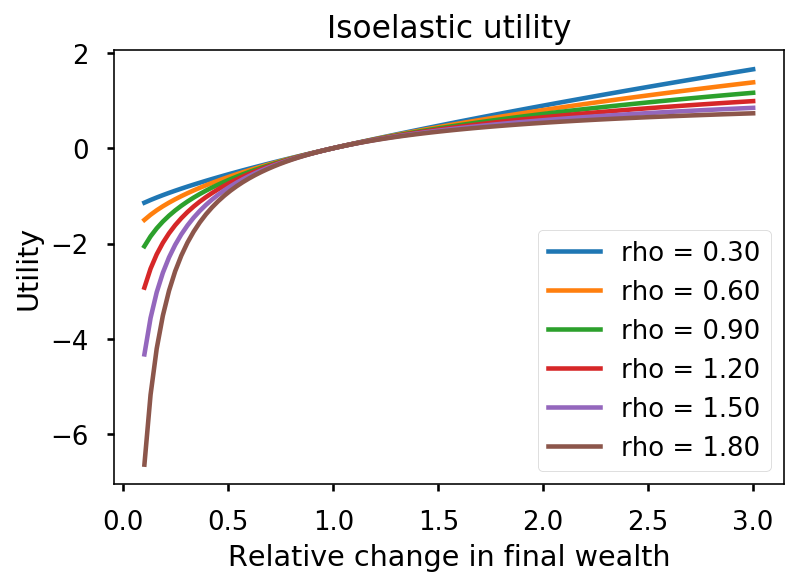
\includegraphics[width=0.7\linewidth]{Thesis/images/isoelastic}
		\caption{Изоэластичная функция полезности}
		\label{fig:isoelastic}	
	\end{figure}
\end{minipage}
\vspace{.5cm}

Это изоэластичная функция полезности. При $\rho=0$ она риск нейтральна, при $\rho \to \infty$ достигается абсолютное избегание риска. Для составления портфеля максимизируется её  матожидание:
\begin{equation}
\Eb[r_w]{U_\rho(r_w)} \to \max_w, \quad w>0,\quad \sum w = 1
\label{eq:isoelastic}
\end{equation}
